% fundDom.tex      pdflatex ZhCvGo15

% Diffuse globally, compute locally: a cyclist tale
% Tingnan Zhang, Daniel I. Goldman and Predrag Cvitanovi\'c

%\section{Into the fundamental domain}
%\label{s-fundDom}

\begin{figure}[htbp]
  \begin{center}
    (a)\;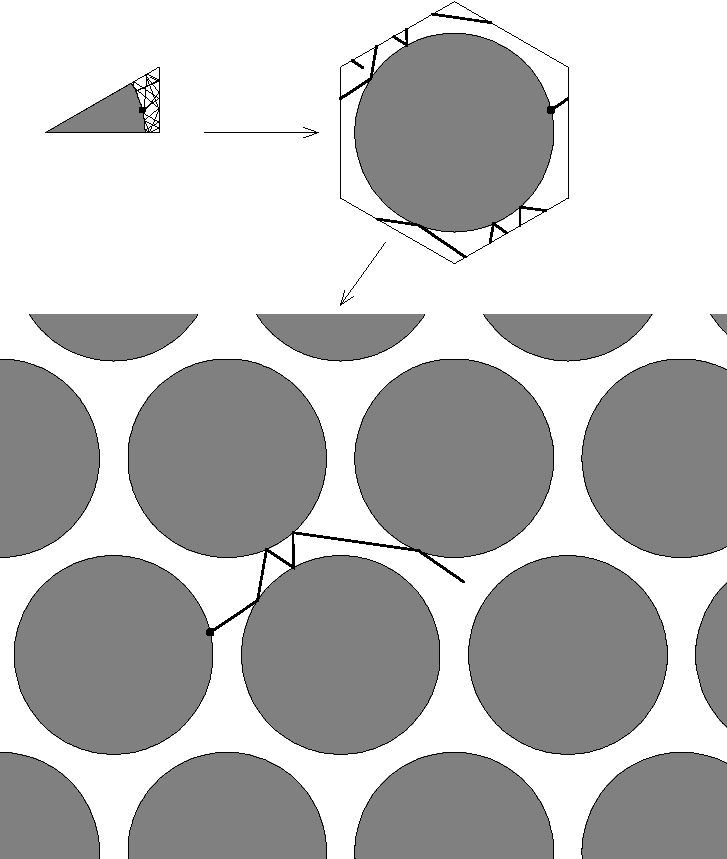
\includegraphics[width=0.43\textwidth]{diffuseSchreiberFig1}
    (b)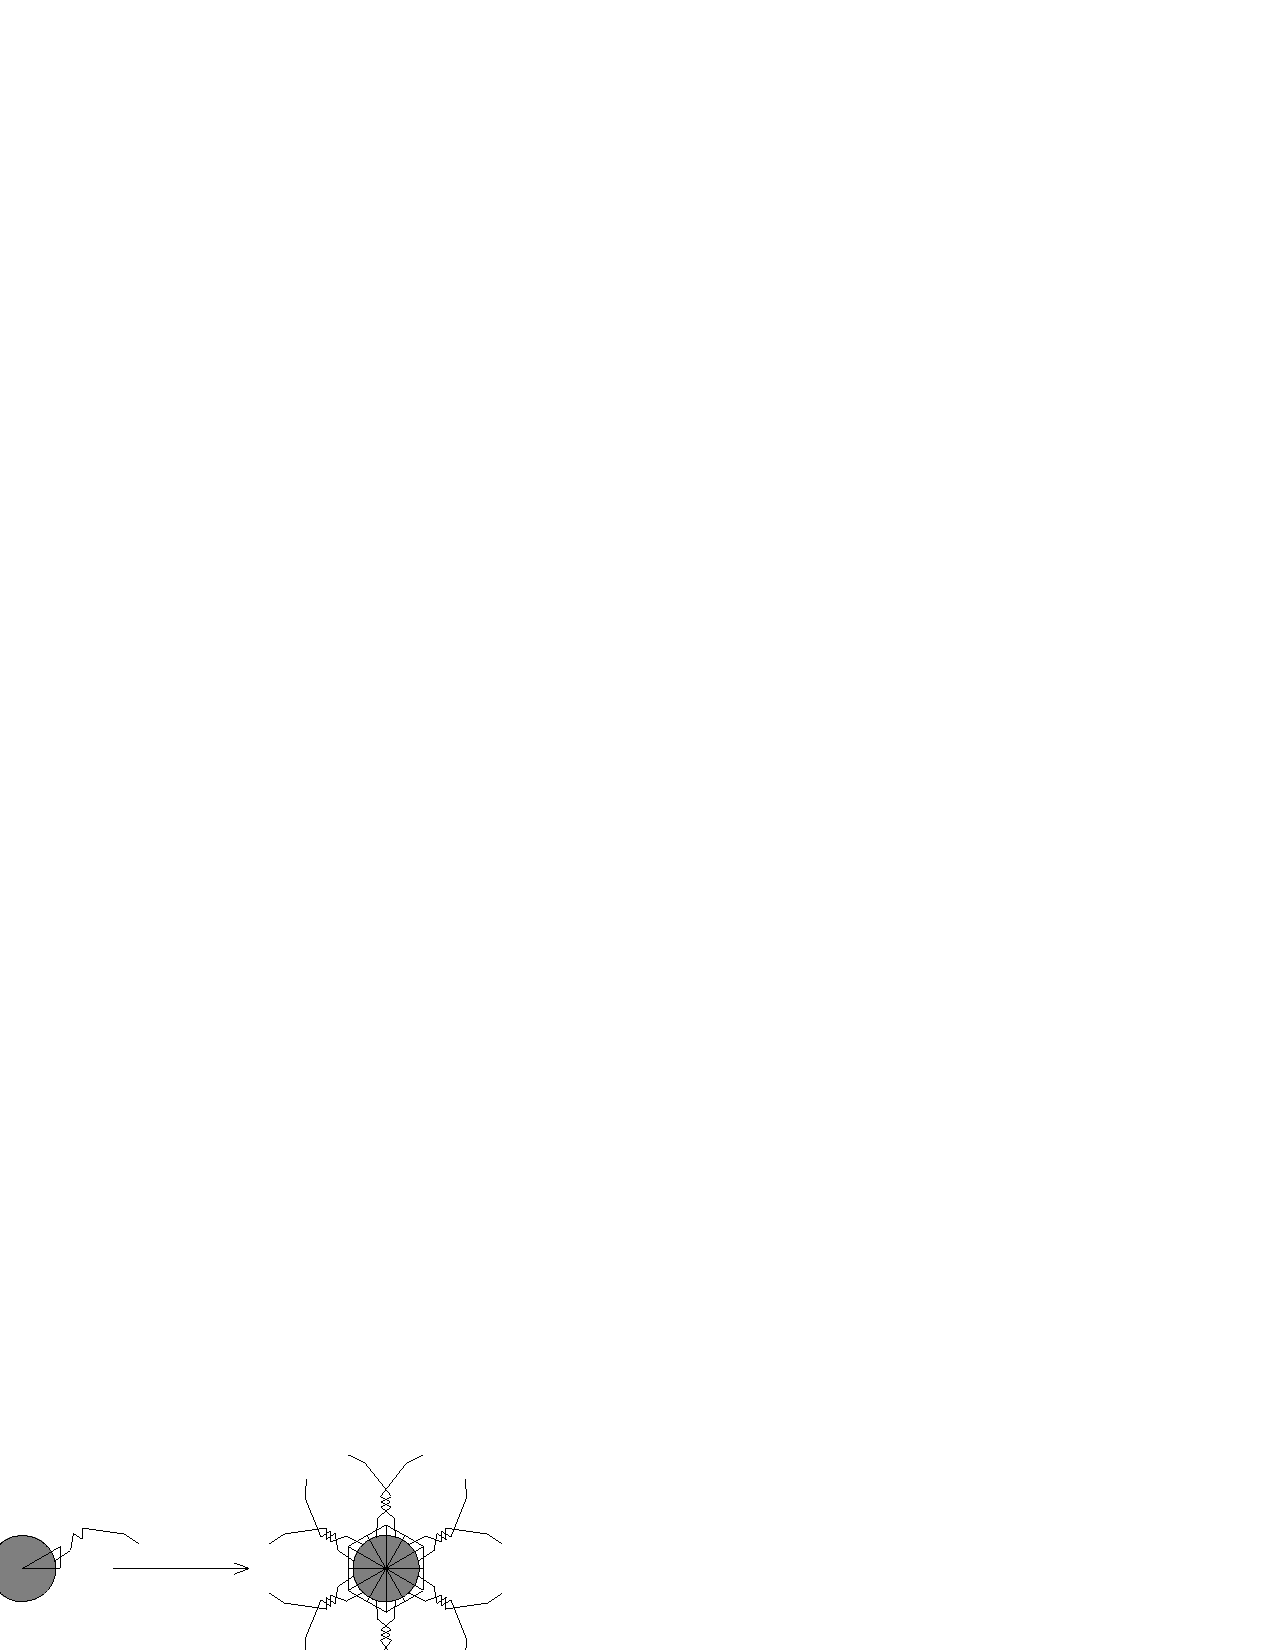
\includegraphics[width=0.45\textwidth]{diffuseSchreiberFig2}
  \end{center}
  \caption[]{\label{fig-schrieberFig12}
  (a) Motion in the fundamental domain (top left), elementary cell (top
      right) and the full space (bottom).
  (b) The above trajectory unwrapped in the full space and its 12 copies
    obtained by applying all point group \Dn{6} actions to it (from
    \refref{CGS92}).
  }
\end{figure}

In addition to translational invariance, many systems bear other type of
symmetries blah, and why we are interested in reduce the symmetry.

The symmetry of the triangular periodic Lorentz gas is the space group
$p6mm$ (see Cotton\rf{Cotton08} {\em Chemical applications of group
theory},  Chapt.~11, for a pretty discussion of the geometry of space
groups). Space group $p6mm$ has a point subgroup $C_{6v}=\Dn{6}$. Leaving
the mathematical representation of group for later discussion, we can
intuitively understand the symmetry by decomposing the hexagonal
elementary cell into 12 identical triangular tiles, as in
\reffig{fig-schrieberFig12}\,(a), upper left, the fundamental domain and
its 11 copies. The fundamental domain tiles the full hexagon, by
application of the \Dn{6} rotations around the center or reflection along
symmetry lines, i.e. the point group actions.

In \refsect{s-Lorentz} we had reduced a trajectory from full space to
elementary cell, as in \reffig{fig-schrieberFig12}\,(a), upper right,
using the translational symmetry, and were able to compute various
quantities in terms of elementary cell \po s. In this section we will
further use the point group symmetry to derive the fully symmetry-reduced
trace formula and, for the first time, the diffusion constant using
cycles restricted to the fundamental domain.

As we will work with three kinds of \statesp s,
we state here what tildes, nothings and hats atop symbols signify:
\bea
\tilde{\ }     &~~&
    \mbox{fundamental domain, triangle in \reffig{fig-schrieberFig12}}
        \continue
%[nothing] \qquad \qquad &&
[0pt] \qquad \qquad &&
    \mbox{elementary cell, hexagon in \reffig{fig-schrieberFig12}}
        \continue
\hat{\ }   &&
    \mbox{full {\statesp}, lattice in \reffig{fig-schrieberFig12}}
\label{atops}
\eea
It is convenient to define an \evOper\ for each of the 3
cases of \reffig{fig-schrieberFig12}.
$\hx(t)\,=\,\hflow{t}{\hx}$
denotes the point in the global space
$\hM$
reached by the flow in time $t$.
$x(t)\,=\,\flow{t}{\xInit}$
denotes the corresponding flow in the elementary cell;
the two are related by
\beq
\hn_t(\xInit)= \hflow{t}{\xInit} - \flow{t}{\xInit} \in T
\,,
\ee{l-diff-hatn}
the translation of the endpoint of the global path into the elementary
cell $\pS$. The quantity $\tx(t)\,=\,\tflow{t}{\tx}$ denotes the flow in
the fundamental domain ${\widetilde \pS}$; $\tflow{t}{\tx}$ is related to
$\flow{t}{\tx}$ by a discrete symmetry $g \in G$ which maps
$\tx(t)\in {\widetilde \pS}$ to ${x}(t) \in {\pS}$.

Starting any point $\ssp$ on a elementary cell cycle $p$, after completing a cycle the particle crosses each cell boundary the same number of times. Because translations are commutative, the particle will always reach the same copy of elementary cell. By eq. \refeq{l-diff-hatn} the total displacement along the cycle is independent of the point of choice. In other words, the displacement is an invariant of the elementary cell cycle. However, when we take into account the point group symmetry (i.e. rotations and reflections), the above statement does not stand. We will need to address the non-commutativity of symmetries and develop new invariants to compute diffusion coefficient.

%\begin{figure}[htbp]
%  \begin{center}
%    (a)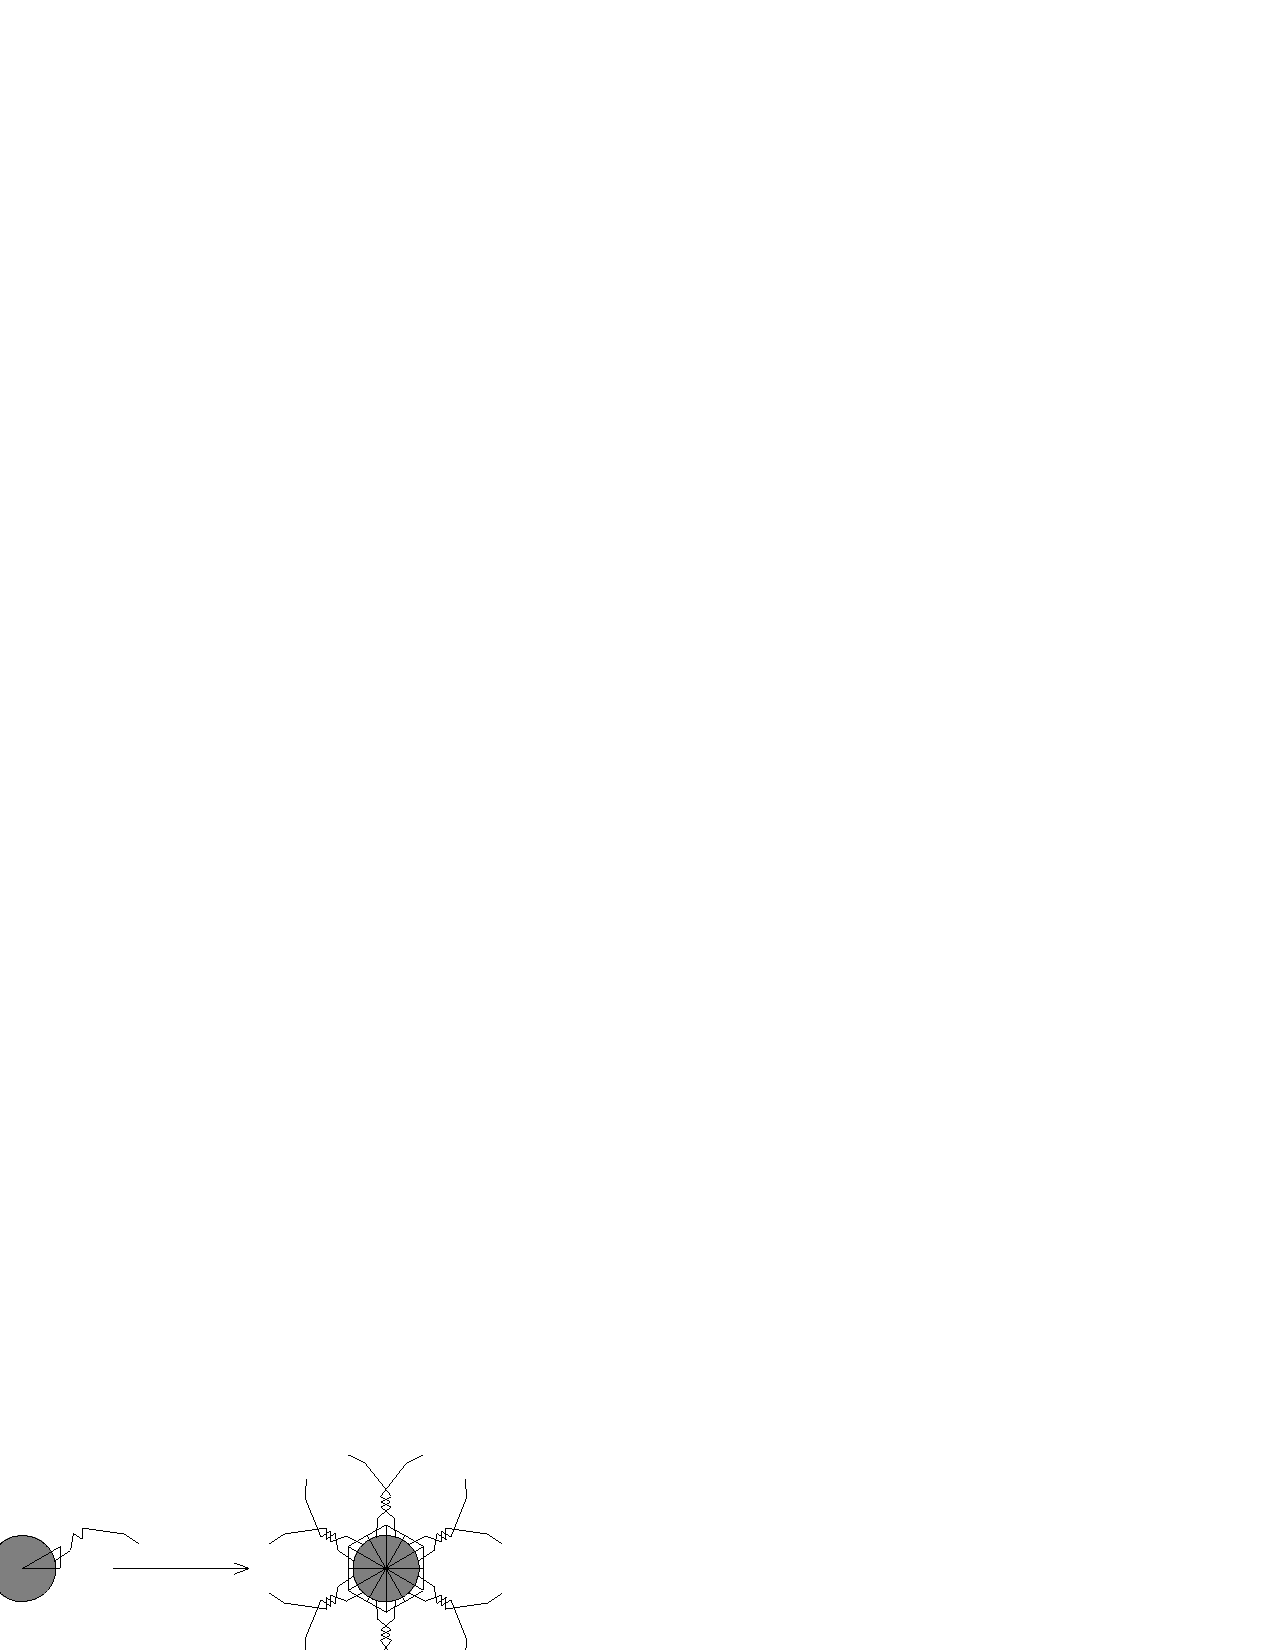
\includegraphics[width=0.45\textwidth]{diffuseSchreiberFig2}
%    (b)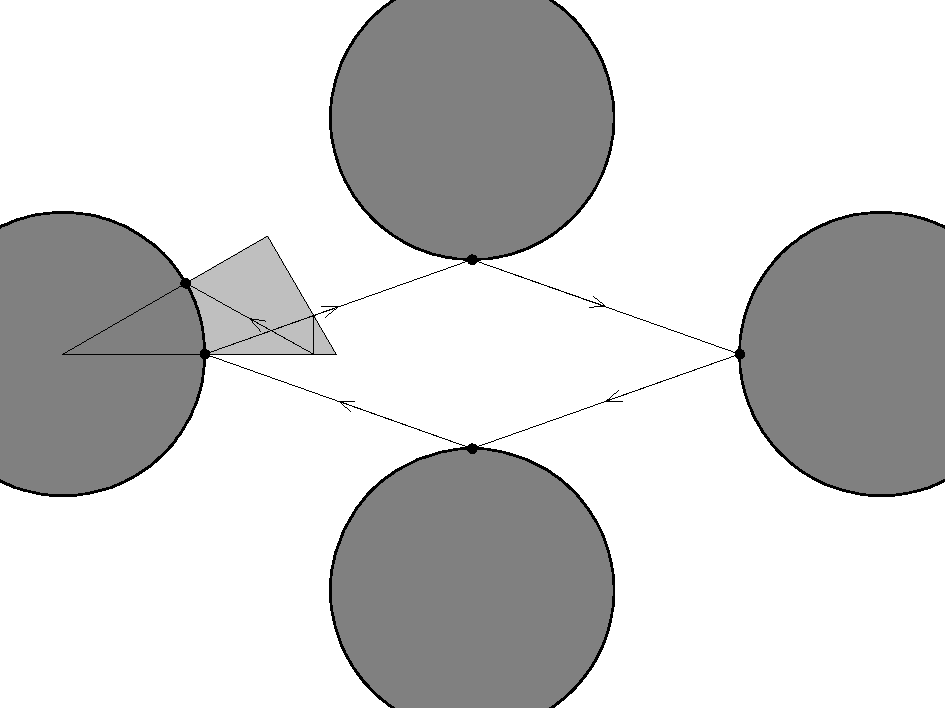
\includegraphics[width=0.45\textwidth]{diffuseSchreiberFig3}
%  \end{center}
%  \caption[]{ \label{fig:schrieberFig23} (a) An (unwrapped) trajectory (in full
%  space) and its 12 copies after applying point group actions to it. (b)
%  Multiplicity of periodic orbits in fundamental domain.}
%\end{figure}

%When the scattering array has a discrete symmetries, such as
%reflection symmetry, each elementary cell may be built from a {\em
%fundamental domain} ${\widetilde \pS}$ by the action of a discrete (not
%necessarily abelian) group $G$. The quantity $\tx(t)\,=\,\tflow{t}{\tx}$
%denotes the flow in the fundamental domain ${\widetilde \pS}$;
%$\tflow{t}{\tx}$ is related to$\flow{}{\tx}$ by a discrete symmetry $g
%\in G$ which maps $\tx(t)\in{\widetilde \pS}$ to ${x}(t) \in {\pS}$. The
%full $\hM \rightarrow {\widetilde\pS}$ reduction is complicated by the
%non-abelian nature of $G$, and will be illustrated in this section in
%detail.

\PC{2016-01-01}{explain that any elementary cycle point translate by the
same amount in the full {\statesp}}

\subsection{Point group changes translation}

While a full space (or elementary cell) trajectory can be uniquely reduced to its fundamental domain counter part by wrapping (reflecting and rotating) all the individual segments in different fundamental domain into a single one, the reverse process is always one-to-many. Because the fundamental domain do not have the concepts of absolute orientation, a single unwrapped trajectory may have up-to 12 isometric copies after we apply the discrete group actions. Even worse, depending on where we start to unwrap the trajectory, the full space trajectories can be completely different in shape. A precise mathematical treatment is necessary to address the above effects, before we can proceed to the complete formula for diffusion, which depends on descriptions of displacements.

We start by first working on the relation of translation and discrete symmetry. A point $\ssp$ in the elementary cell is identified by its
fundamental domain mirror image:
\[ %beq
\ssp=g\,\tx,
\] %eeq
given a group action $g\in G$. We have to appreciate that both the full space flow $\hflow{t}{\ssp}$ and elementary flow $\flow{t}{\ssp} $ is G-equivariant under the lattice group symmetry,.
\[
\hflow{t}{g\,\tx} = g\,\hflow{t}{\tx}\,,
\flow{t}{g\,\tx} = g\,\flow{t}{\tx}
\]

Then the displacement in full space is also G-equivariant:
\[ %beq
\hn_t(\ssp)= \hflow{t}{g\,\tx} - \flow{t}{g\,\tx}=g\,(\hflow{t}{\tx} - \flow{t}{\tx}) = g\,\hn_t(\tx)\,.
\] %eeq

We apply this rule to the displacement associated with a prime
periodic orbit $\tp$ restricted in the fundamental domain.
Let $\tp\equiv\{\tx_0,\tx_1,\ldots,\tx_{\cl{\tp}}\}$, with topological length
$\cl{\tp}$ and $\tx_i$ the bouncing points on the orbit.


For each free flight (\eg, from $\tx_i$ to $\tx_{i+1}$) we denote the associated
displacement in full space $\hn(\tx_i,e)$. Special caution has to be
taken when we add the individual displacements together as the particle moves
along a fundamental domain orbit. Each time the particle crosses a boundary (the
symmetry lines), it is deflected back in the same domain as if it hits a wall.
However, in the elementary cell the particle has already entered another triangular pieces, and we have to record the associated group actions that can maps it back. Before the next collision, we assign $g_\tp(\tx_{i+1},\tx_{i})$  as the total group element during the flight to keep track of changes in absolute orientation. We can now write the displacement traveled along the orbit, after finishing a full cycle:
\beq
\hn_{\tp}(\tx_{0})=\sum_{i=0}^{\cl{\tp}-1}\hn(\tx_{i},g_{\tp,\tx_0}(\tx_{i}))
=\sum_{i=0}^{\cl{\tp}-1}g_{\tp,\tx_{0}}(\tx_{i})\,\hn(\tx_{i},e),
\eeq
where $g_{\tp,\tx_{0}}(\tx_i)=\prod_0^{j-1} g_\tp(\tx_{j+1},\tx_{j})$ is
the accumulated orientation changes along the orbit when starting from
$\tx_{0}$. The displacement has an explicit dependence on starting point. We denote the total group action (orientation change) for the orbit
\bea
h_{\tp}(\tx_i)&\equiv& g_\tp(\tx_{i},\tx_{i-1})\,\ldots\,
g_\tp(\tx_{0},\tx_{\cl{\tp}-1})\nonumber\\
&& \, g_\tp(\tx_{\cl{\tp}-1},\tx_{\cl{\tp}-2})\, \ldots\,
g_\tp(\tx_{i+1},\tx_{i}),
\eea

which also immediately connects the flow in fundamental domain and elementary cell by
\[\flow{t_\tp}{\tx_i}=h_{\tp}(\tx_i)\tflow{t_\tp}{\tx_i}.\]

Although the group action $h_{\tp}(\tx_i)$ depends on the initial points
on the orbit as well, it is a property of the orbit's symmetry. One can easily show that all $h_{\tp}(\tx_i), \tx_i\in\tp$ belong to the \emph{same} subgroup of $G$.


If we let the particle (starting from $\tx_i$) travel along the fundamental domain orbit $r$ times, the cumulated displacement is then given by:
\beq
\hat{L}_{\tp}^{r}(\tx_i)\equiv
(e+\hp^{1}(\tx_i)+\cdots+\hp^{r-1}(\tx_i))\cdot\hn_{\tp}(\tx_i),
\label{eq-fdDisplacement}
\eeq
